\section{Cylc Introduction}
\label{Cylc Introduction}

\note{For more information on the topics of this section, see Appendix~\ref{Appendix
Cylc Introduction} and the Cylc User Guide.}

\subsection{The suite.rc File}

A cylc suite is a collection of files in a {\em suite directory} configured by
a single {\em suite.rc} file, which is written in a nested INI format with
section and sub-section (etc.) headings denoted by square brackets.

\begin{lstlisting}[language=suiterc]
[section]
    option = value
    [[sub-section]]
        option = value
\end{lstlisting}

The most important top level sections in a suite.rc file are:

\begin{tabular}{ll}
\begin{lstlisting}
[cylc]
\end{lstlisting} & various suite-level settings\\
\begin{lstlisting}
[scheduling]
\end{lstlisting} & determines {\em when} tasks are ready to run (e.g.\ dependencies)\\
\begin{lstlisting}
[runtime]
\end{lstlisting} & defines {\em what} to run when a task is ready, and
{\em where} and {\em how} to run it \\
\end{tabular}


\subsection{Hello World in cylc}

This suite runs a single task named \lstinline{hello} that prints ``Hello
World!'', sleeps for a few seconds, then exits:

% Call task just "hello" to distinguish the task name from the suite name.
% Sleep for 30 seconds - long enough to be seen in the GUI.

\begin{lstlisting}[language=suiterc]
[scheduling]
    [[dependencies]]
        graph = hello
[runtime]
    [[hello]]
        script = echo "Hello World!"; sleep 30
\end{lstlisting}

The \lstinline{[scheduling]} section says to run the hello task immediately on
start-up, because it doesn't depend anything else; and the
\lstinline=[runtime]= section says that the task should run the given inlined
shell scripting.

You can run a new cylc suite like this (but don't do it just yet):

\begin{lstlisting}[language=bash]
$ cylc register hello_world /path/to/hello_world/  # register name "hello_world"
$ cylc validate hello_world  # check for configuration errors
$ cylc run hello_world  # run the suite
$ cylc gui hello_world &  # open a suite control GUI
\end{lstlisting}

In this tutorial however, we will be using the \lstinline{rose suite-run},
command to run suites.  It automatically installs, registers, validates, starts
the suite with \lstinline=cylc run=, and opens the cylc GUI.

The \lstinline{cylc run} command starts a new {\em suite daemon} to run your
suite.  It will stay alive even if you log out, until your suite runs to
completion or you tell it to shut down.

\terminology{A cylc \underline{suite daemon} is a light-weight server program
dedicated to managing a single workflow.}

\subsection{Hello World Tutorial}

\begin{shaded*}

Copy the Hello World example code above into a {\em suite.rc} file in a directory called
{\em hello\_world}, and run the following commands:

\begin{lstlisting}[language=bash]
$ cd hello_world  # move to the suite directory
$ touch rose-suite.conf  # create an empty rose-suite.conf file
$ rose suite-run  # install, register, validate, run the suite, and open the GUI
\end{lstlisting}

If no errors are found in the suite.rc file your suite will start up and a
GUI window will appear showing the \lstinline{hello} task with a coloured
square representing its state. For example, green means `running' and gray
`succeeded'.  Once the task has succeeded, the suite has no more tasks to run
and will shut down.

Note that ``Hello World!'' is not printed to the terminal. It is printed by 
the \lstinline=hello= task, which is launched by the suite daemon as a separate
process (potentially on another machine, although not in this case).

\terminology{A task \underline{job script} is a shell script generated by cylc
    to run a task as defined in the suite.rc file.}

The job script and its output are written to a standard job log directory:

\begin{lstlisting}[language=bash]
$ ls -1 $HOME/cylc-run/hello_world/log/job/1/hello/01/
job  # task job script
job.out  # task standard out
job.err  # task standard error
job.status
job-activity.log
\end{lstlisting}

The task job logs are automatically retrieved to the suite host, if the task
runs on another machine.

While a task is visible in the GUI, right-click on it to view its log files.
After that, look in its log directory:

\begin{lstlisting}[language=bash]
$ cd $HOME/cylc-run/hello_world/log/job/1/hello/01/
$ cat job.out
...
Hello World!
...
\end{lstlisting}

or use the \lstinline{cylc cat-log} command:

\begin{lstlisting}[language=bash]
$ cylc cat-log --help  # see "cylc --help" for top level command help
$ cylc cat-log --stdout hello_world hello.1
...
Hello World!
...
\end{lstlisting}

or use the \lstinline{rose suite-log} web-based suite log file viewer:

\begin{lstlisting}[language=bash]
$ cd hello_world
$ rose suite-log
# (now view suite and job logs in your web browser)
\end{lstlisting}

\end{shaded*}

\subsection{Defining Tasks}

A task can run an external program or script, or shell scripting
inlined in the suite.rc file, or any combination of the two.  A suite
\lstinline{bin} directory is automatically added to your shell
\lstinline{$PATH} so that scripts residing in it can be called by name,

% changed original script name 'get-host-details' - users may wonder if host
% details are somehow communicated back to the suite.
\begin{lstlisting}[language=suiterc]
[runtime]
    [[model]]
        script = run-model  # in <suite-dir>/bin/ (or elsewhere in $PATH)
\end{lstlisting}

or use a full file path,

\begin{lstlisting}[language=suiterc]
[runtime]
    [[model]]
        script = /path/to/my-scripts/run-model
\end{lstlisting}

or set \lstinline{$PATH} in the task environment (this makes more sense
if the environment is inherited by multiple tasks - see
Section~\ref{Families}),
\begin{lstlisting}[language=suiterc]
[runtime]
    [[model]]
        script = run-model
        [[[environment]]]
            PATH = /path/to/my-scripts:$PATH
\end{lstlisting}

You can pass information to a script via its command line or environment,

\begin{lstlisting}[language=suiterc]
[runtime]
    [[model]]
        script = run-model --color=green
        [[[environment]]]
            START_TIME = $CYLC_TASK_CYCLE_POINT
\end{lstlisting}

or use custom multi-line scripting, in triple quotes, to do anything you like:
\begin{lstlisting}[language=suiterc]
[runtime]
    [[model]]
        script = """
cat > model-input.txt <<__EOF__
COLOR=green
START_TIME=$CYLC_TASK_CYCLE_POINT
__EOF__
run-model model-input.txt"""
\end{lstlisting}

An optional \lstinline=[[[remote]]]= section determines {\em where} a task
will run (defaults to localhost), 

\begin{lstlisting}[language=suiterc]
[runtime]
    [[model]]
        script = run-model
        [[[remote]]]
            host = supercomputer
\end{lstlisting}
(In this case the \lstinline=run-model= script and any files that it needs -
such as the model program itself - must be installed on host ``supercomputer'').

An optional \lstinline=[[[job]]]= sub-section determines {\em how} the task
should be submitted to run (defaults to ``background'', an ordinary shell
subprocess).
\begin{lstlisting}[language=suiterc]
[runtime]
    [[model]]
        script = run-model
        [[[job]]]
            batch system = pbs
\end{lstlisting}

\note{So far we have only configured individual tasks.  In fact the
\lstinline=[runtime]= section is a {\em multiple inheritance hierarchy} that
allows all shared configuration to be factored out into {\em families} that are
inherited by multiple tasks - see Section~\ref{Families}.} 

\subsection{Dependency Graphs}

The hello\_world suite contained the {\em graph string}
\lstinline@graph = hello_world@.  Graph strings specify the scheduling logic
that determines when tasks can run: which tasks depend on, or {\em trigger off},
which other tasks, if any.  For instance if we have two tasks \lstinline{foo}
and \lstinline{bar}, and \lstinline{foo} depends on \lstinline{bar} succeeding,
we could write:

\begin{lstlisting}[language=suiterc]
graph = "foo:succeed => bar"
\end{lstlisting}

If \lstinline{foo} fails here, \lstinline{bar} will not run.  Tasks can also
trigger off failure and other conditions, but success triggers are the default
so \lstinline=:succeed= can optionally be omitted:

\begin{lstlisting}[language=suiterc]
graph = "foo => bar"
\end{lstlisting}

A graph string can contain many triggers, and the default success triggers can
be chained together. This,

\begin{lstlisting}[language=suiterc]
graph = "foo => bar => baz"
\end{lstlisting}

is equivalent to this,

\begin{lstlisting}[language=suiterc]
graph = """foo => bar
           bar => baz"""
\end{lstlisting}

You can also write conditional triggering logic with \lstinline=&= (AND) and
\lstinline=|= (OR) operators. For example,

\begin{lstlisting}[language=suiterc]
graph = "foo => bar & baz"  # foo => bar, AND foo => baz
\end{lstlisting}

The \lstinline=cylc graph= command generates nice suite graph visualizations.
For this graph string,

\begin{lstlisting}[language=suiterc]
graph = """foo => bar => baz & qux => pin
           wol"""
\end{lstlisting}

it produces,

\begin{center}
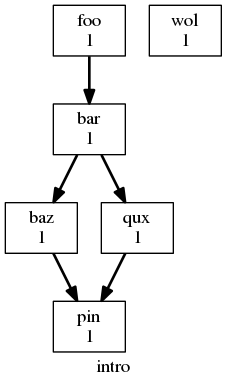
\includegraphics[width=0.2\columnwidth]{resources/intro-1.png} %tex/cylc-graph}
\end{center}

\subsection{Cycling Workflows}

The concept of a workflow of cycling tasks was introduced in Section~\ref{Cylc
Overview}.  The following diagram shows the previous workflow (minus the lone
`wol' task) repeated for three integer cycle points 1, 2 and 3.

\begin{center}
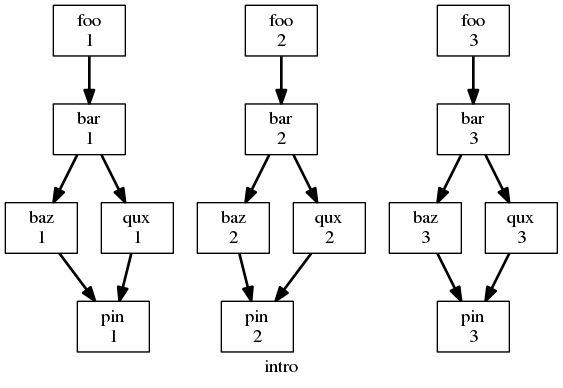
\includegraphics[width=0.5\columnwidth]{resources/intro.png} %tex/cylc-cycle-graph}
\end{center}

In cylc these are three distinct workflows that can run concurrently (which is
how it should be if there is no dependence between them!). In fact many more
than three cycle points could run concurrently, but we deliberately limit the
amount of ``runahead''. The default is:
\begin{lstlisting}
[scheduling]
    max active cycle points = 3
\end{lstlisting}

A cycling suite needs an {\em initial cycle point} and at least one cycling
sequence with associated dependencies defined in a graph string. An optional
{\em final cycle point} can also be given.

\begin{lstlisting}[language=suiterc]
[cylc]
    cycle point format = %Y-%m
[scheduling]
    initial cycle point = 2000-01
    final cycle point = 2000-05
    [[dependencies]]
        [[[P1M]]]
            graph = model
\end{lstlisting}
This suite definition says to run task \lstinline=model= for each cycle point
on a sequence of date-times with a 1-month interval between 2001-01 and 2001-05 
(see~\ref{advanced-cycling} for other kinds of cycling sequence).
With no clock-triggers defined (see~\ref{Clock Triggered Tasks}) these
date-times have no connection to the real-time clock.  Each instance of
\lstinline=model= is merely labelled with its cycle point value (which the task
job can use, e.g.\ as a model run start date).  In this case
there is no dependence between successive \lstinline=model= instances, so they
can all run concurrently, out to \lstinline=max active cycle points=.

\subsection{Inter-Cycle Dependence}

If each instance of \lstinline=model= in the previous example really depends
on its own previous instance (for restart files, say), running multiple
models concurrently would result in failure.  Here's how to express this
inter-cycle dependence correctly,

\begin{lstlisting}[language=suiterc]
[cylc]
    cycle point format = %Y-%m
[scheduling]
    initial cycle point = 2000-01
    final cycle point = 2000-05
    [[dependencies]]
        [[[P1M]]]
            graph = model[-P1M] => model
\end{lstlisting}

\lstinline=P1D= is an ISO8601 duration - see
    \url{http://wikipedia.org/wiki/ISO_8601#Durations}. \lstinline=P= denotes a
    duration and \lstinline=1M= means one month. Other examples of ISO8601
    durations are:
\begin{itemize}
    \item \lstinline{-PT12H} (12 hours ago).
    \item \lstinline{-PT6H30M} (6 hours 30 minutes ago).
    \item \lstinline{P1W} (1 week in the future).
\end{itemize}

\subsection{Cycling Suite Tutorial}

\begin{shaded*}

This demo is an example of a cycling workflow, to run it create a new
directory and create a blank rose-suite.conf file within it.

Next copy the following code into a suite.rc and a bin/count-down file.

\begin{lstlisting}[language=]
|-- bin/
|   `-- count-down
|-- rose-suite.conf
`-- suite.rc
\end{lstlisting}

\begin{lstlisting}[language=suiterc, title=suite.rc]
[scheduling]
    initial cycle point = 2000-01-01T00
    final cycle point = 2000-01-05T00
    [[dependencies]]
        [[[T00]]]
            graph = """
                blast_off[-P1D] => point_upwards
                point_upwards => load_astronauts
                point_upwards => fill_fuel_tank
                point_upwards => set_coordinates
                fill_fuel_tank => light_fuse
                set_coordinates => count_down
                light_fuse => count_down
                load_astronauts => count_down
                count_down => blast_off
            """
[runtime]
    [[point_upwards]]
        script = sleep 2; echo "spikey end pointing at sky, flamey end \
                    pointing at ground"
    [[load_astronauts]]
        script = sleep 1; echo "loaded astronauts"
    [[fill_fuel_tank]]
        script = sleep 5; echo "tank brimmed"
    [[set_coordinates]]
        script = echo "coordinates set for west wallaby st"
    [[light_fuse]]
        script = echo "stand well back"
    [[count_down]]
        script = count-down
    [[blast_off]]
        script = echo "blast off"
\end{lstlisting}

\begin{lstlisting}[language=bash, title=bin/count-down]
sleep 1; echo 5;
sleep 1; echo 4;
sleep 1; echo 3;
sleep 1; echo 2;
sleep 1; echo 1;
\end{lstlisting}

To run this demo suite, enter the following commands:

\begin{lstlisting}[language=bash]
$ chmod +x bin/count-down  # Make the count-down script executable.
$ rose suite-run
\end{lstlisting}

Again a window should open up showing you the progress of the suite.
Whilst the suite is running try entering graph mode by selecting
\lstinline[language=]{View > 1 - Graph View} from the menubar, this will show
the dependencies between the tasks as they run.

\end{shaded*}
